\clearpage

% Customize section counter
\renewcommand\thesection{\arabic{chapter}.\Alph{section}}
\setcounter{section}{0}
\section{Supplementary material}
\label{sec:2_supplement}

% Customize figure counter
\renewcommand{\thefigure}{2.A\arabic{figure}}
\setcounter{figure}{0}

% \subsection{test subsection}

% TODO: negative x-axis
% Figure 2.S1 (percentages)
% -------------------------
\begin{figure}[!tbh]
    \centering
    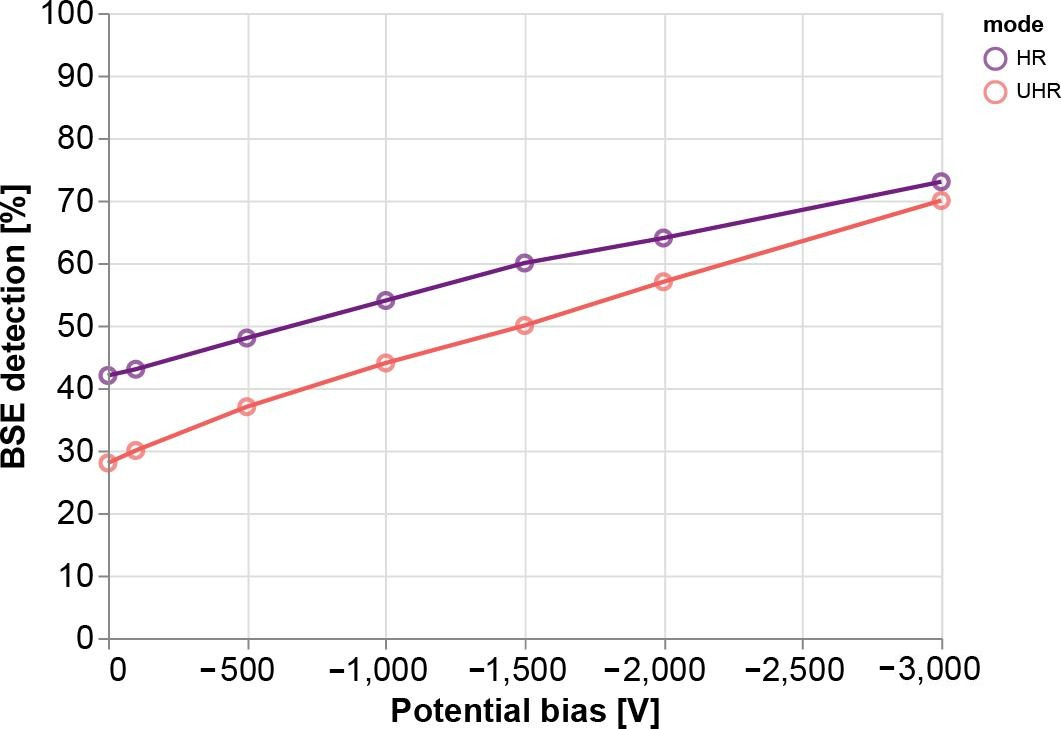
\includegraphics[width=0.75\linewidth]{chapter-2/figures_JPEG_HQ/fig2-S1_percentages.jpg}
    \caption{BSE collection efficiency increases monotonically down to \SI{-3}{\kilo\volt} potential bias for both non-immersion (HR) and immersion (UHR) imaging modes.}
    \label{fig:2.S1_percentages}
\end{figure}



% TODO: caption
% Figure 2.S2 (comparison)
% ------------------------
\begin{figure}[!tbh]
    \centering
    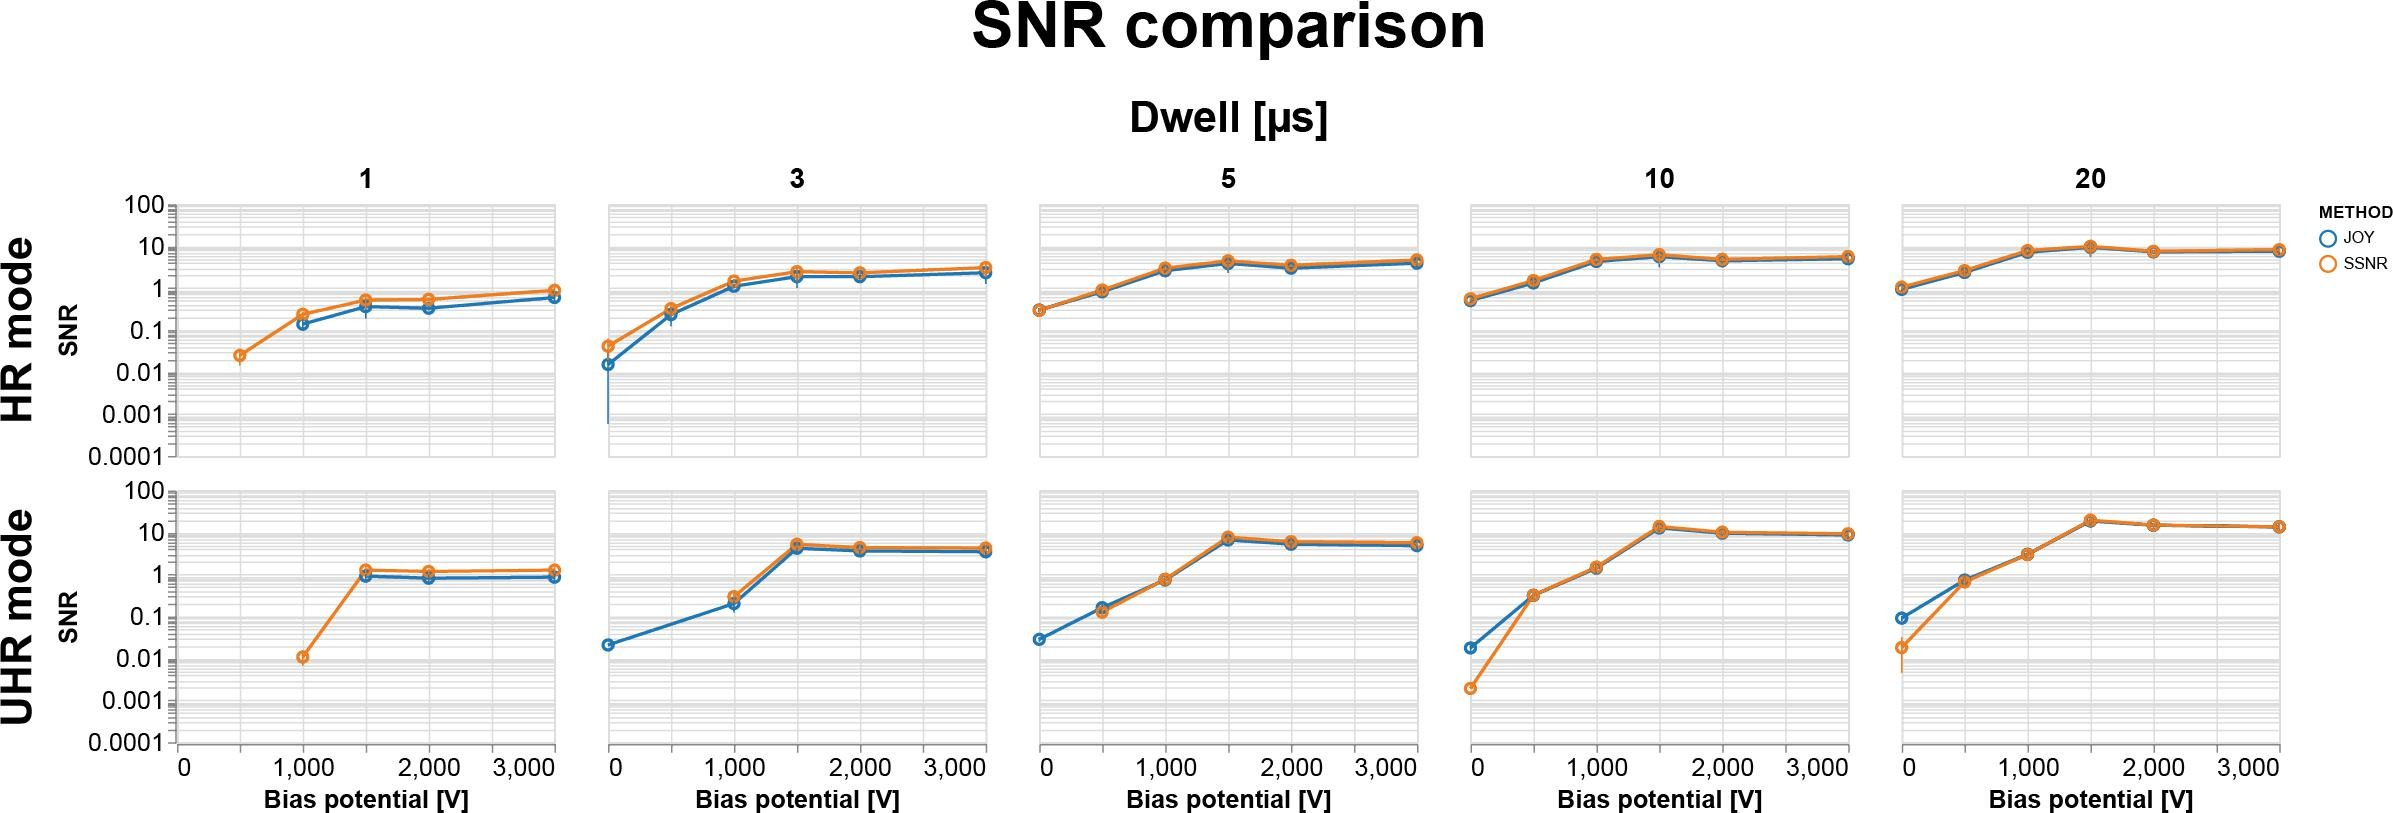
\includegraphics[width=\linewidth]{chapter-2/figures_JPEG_HQ/fig2-S2_comparison.jpg}
    \caption{Comparison between SNR measurements from SSNR-based method and cross-correlation method presented in \textcite{joy2002smart}. The two methods tend to agree with one another for bias voltages below \SI{-500}{\volt}.}
    \label{fig:2.S2_comparison}
\end{figure}
